\documentclass{standalone}
\usepackage{tikz}
\usepackage{pgfplots}
\pgfplotsset{compat=1.11}

\begin{document}
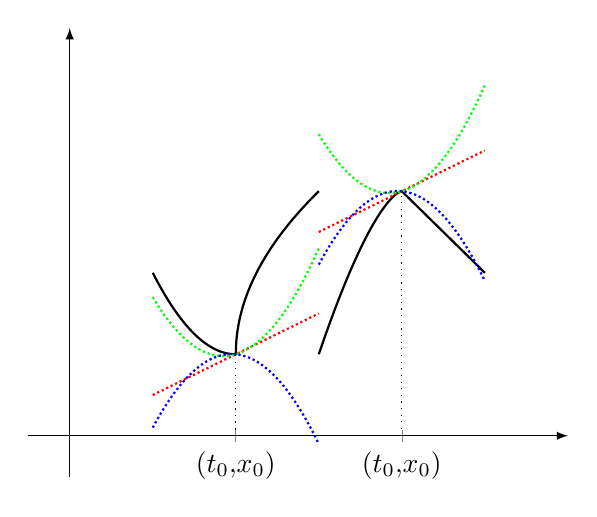
\begin{tikzpicture}
\begin{axis}[ 
axis lines=middle,
xmin=0,
xmax=5.5,
ymin=0,
ymax=4.5,
    axis lines=middle,
        enlargelimits={abs=0.5},
    axis line style={-latex},
%xlabel={$(t,x)$},          % default put x on x-axis
%                    xticklabels={},
%                    xtick={1},     
                                     xticklabels={$(t_0{,}x_0)$,$(t_0{,}x_0)$},
                    xtick={2,4},        
                   ytick=\empty,
]
\addplot[thick,domain=2:3,samples=200] ({x},{1+2*sqrt(abs(x-2))});
\addplot[thick,domain=1:2.01,samples=200] ({x},{1+(x-2)^2)});
\addplot[thick,densely dotted,red,domain=1:3,samples=200] ({x},{1+0.5*(x-2))});
\addplot[thick,densely dotted,green,domain=1:3,samples=200] ({x},{1+0.3*(x-2)+(x-2)^2)});
\addplot[thick,densely dotted,blue,domain=1:3,samples=200] ({x},{1-0.1*(x-2)-(x-2)^2)});
\addplot[dotted,domain=0:1] ({2},{x});


\addplot[thick,domain=3:4,samples=200] ({x},{3-2*sqrt(abs(x-4))^3});
\addplot[thick,domain=5:3.99,samples=200] ({x},{3-(x-4))});
\addplot[thick,densely dotted,red,domain=3:5,samples=200] ({x},{3+0.5*(x-4))});
\addplot[thick,densely dotted,green,domain=3:5,samples=200] ({x},{3+0.3*(x-4)+(x-4)^2)});
\addplot[thick,densely dotted,blue,domain=3:5,samples=200] ({x},{3-0.1*(x-4)-(x-4)^2)});
\addplot[dotted,domain=0:3] ({4},{x});

\end{axis}
\end{tikzpicture}

\end{document}